アルゴリズムを実装し、各データセットにおけるアルゴリズムの実行時間をそれぞれ示す。実験環境は
\begin{description}
  \item[OS] Mac OS X El Caption (10.11.6)
  \item[CPU] Intel(R) Core(TM) i7-3770 CPU @ 3.40GHz
  \item[Memory] 16GB 1600MHz DDR3
\end{description}
でおこない、
\begin{algorithm}
  \caption{$\epsilon > 0$の与え方}
  \begin{algorithmic}
    \For {$i = 1$ to $10$}
      \For {$j = 9$ to $1$}
        \State $\epsilon = j \times 10^{-i}$
        \For {$k = 1$ to $100$}
          \State Main Procedureを$\epsilon$と実験で用いる$A_1, A_2, \cdots, A_m$を引数に呼び出し、実行時間を計測
        \EndFor
      \EndFor
    \EndFor
  \end{algorithmic}
\end{algorithm}
として、Forループ1反復ごとの$\epsilon$とともにMain Procedureを100回呼び出してMain Procedureの実行時間から平均実行時間を算出した。実装はMATLAB 2016bを用いて行った。

\subsection{実験1}
\begin{align*}
  A_1 & = \left(
            \begin{array}{ccc}
              2 &  0 &  0 \\
              0 &  0 & -1 \\
              0 & -1 &  0
            \end{array}
          \right) \\
  A_2 & = \left(
            \begin{array}{ccc}
              0 & 0 & 0 \\
              0 & 1 & 0 \\
              0 & 0 & 0
            \end{array}
          \right) \\
  A_3 & = \left(
            \begin{array}{ccc}
              0 & 0 & 1 \\
              0 & 0 & 0 \\
              1 & 0 & 0
            \end{array}
          \right) \\
  A_4 & = \left(
            \begin{array}{ccc}
              0 & 1 & 0 \\
              0 & 0 & 0 \\
              0 & 0 & 0
            \end{array}
          \right)
\end{align*}
を条件として使用して実験を行った。この実験では双対問題の許容解
\begin{align} \label{test1-results}
  \displaystyle{\sum_{i = 1}^4} u_i A_i \succ 0\text{となる}\mathbf{u}
\end{align}
がアルゴリズムの結果として得られる。実際に得られた実験結果は図\ref{test1}のようになっている。
\begin{figure}
  \centering
  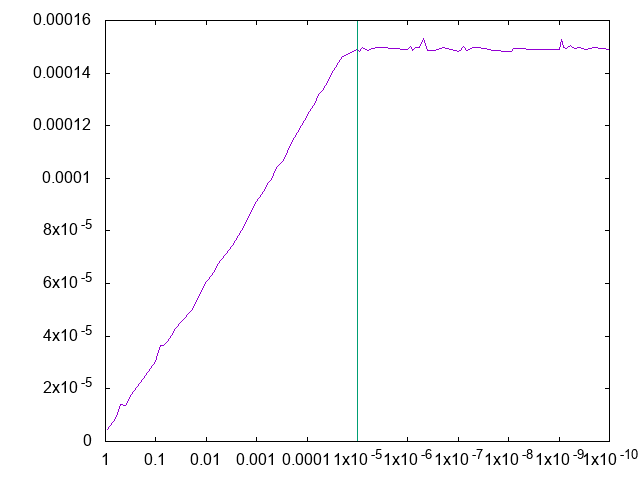
\includegraphics[width=10cm]{test1.png}
  \caption{実験1の実験結果}
  \label{test1}
\end{figure}

理論的には問題(\ref{SemidefiniteSystem})の許容解は出ずに、双対問題の許容解(\ref{test1-results})が結果として得られるはずであるが、$\epsilon$が大きい間はMain Procedureが先に終了してしまうため、アルゴリズムが解までたどり着くことができない。しかし、ある程度$\epsilon$が小さくなるとMain Procedureも十分な回数分反復することができるようになるため、理論的な結果と一致するようになったと考えられる。実際、図中の縦棒である、$10^{-5}$以降は理論的な結果と一致して双対問題の許容解(\ref{test1-results})が得られた。これ以降はどれほど$\epsilon$を小さくしようとも、双対問題の許容解(\ref{test1-results})が得られるため、実行時間が一定になっている。

\subsection{実験2}
\begin{align*}
  A_1 & = \left(
            \begin{array}{ccc}
              0 &  0 &  0 \\
              0 &  1 & -1 \\
              0 & -1 &  0
            \end{array}
          \right) \\
  A_2 & = \left(
            \begin{array}{ccc}
              0 & 0 & 0 \\
              0 & 1 & 0 \\
              0 & 0 & 0
            \end{array}
          \right) \\
  A_3 & = \left(
            \begin{array}{ccc}
              0 &  0 &  0 \\
              0 & -1 &  0 \\
              0 &  0 & -2
            \end{array}
          \right) \\
\end{align*}
を条件として使用した。この実験では双対問題の解(\ref{test1-results})や、問題(\ref{SemidefiniteSystem})の許容解$X \succ 0$は得ることができない。実際に得られた結果は図\ref{test2}の通りである。
\begin{figure}
  \centering
  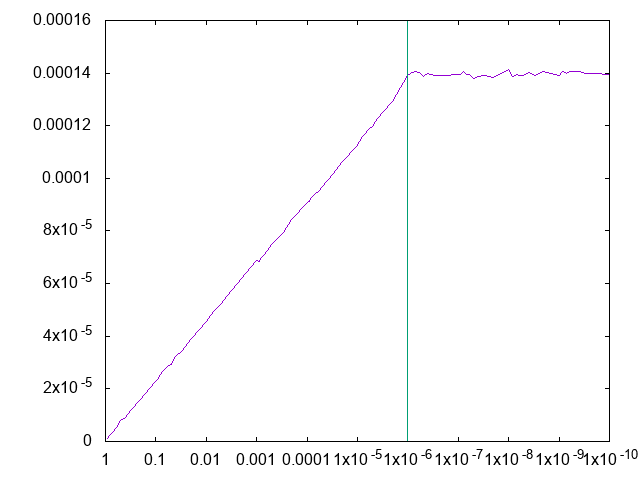
\includegraphics[width=10cm]{test2.png}
  \caption{実験2の実験結果}
  \label{test2}
\end{figure}

この実験ではアルゴリズムは双対問題の許容解(\ref{test1-results})や、問題(\ref{SemidefiniteSystem})の許容解$X \succ 0$を得ることはできない。今回の実装として、100回Main Procedureが反復を行った場合、強制的にアルゴリズムを終了するようになっている。そのため、$10^{-6}$以降はこの最大反復回数を超えてしまうため、一定の実行時間しか得られなかった。

\subsection{実験3}
$50$次実対称行列を30個用意した。各要素の値はpythonのメルセンヌツイスタを用いて$[-10,10]$の範囲で生成した整数を用いている。

実験結果は図\ref{randomtest}のようになった。
\begin{figure}
  \centering
  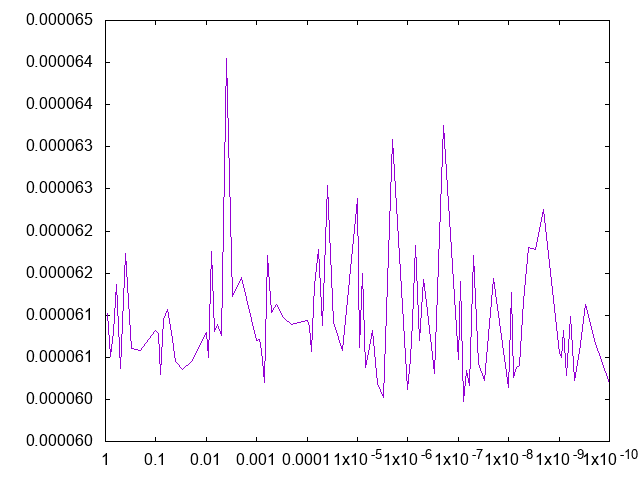
\includegraphics[width=10cm]{randomtest.png}
  \caption{実験3の実験結果}
  \label{randomtest}
\end{figure}
この実験では$\epsilon$がどのような値であっても問題(\ref{SemidefiniteSystem})の許容解$X \succ 0$がみつかる。しかし、前述の実験のように$\epsilon$の値に応じて常に実行時間線形の値となるわけではなく、起伏が激しくなってしまった。これは実行時間が短かすぎたために、コンテキストスイッチなどのアルゴリズムとは本質的には関係ない実行時間による影響が大きくなってしまったのではないかと考えられる。
